\documentclass[10pt,times]{beamer}
\usepackage{amsfonts}
\usepackage{amsmath}
\usepackage{amssymb}
\usepackage{mathptmx}

\usepackage{color}
\usepackage{minted}
\usepackage{hyperref}
\usepackage{multicol}
\usepackage{multirow}
\usepackage{tabularx}
\usepackage{booktabs}
\usepackage{menukeys}
\usepackage{subcaption}

% ******************************** Meta-data ***********************************
\mode<presentation>
{
  \usetheme{Madrid}
  \setbeamercovered{transparent}
}


\usepackage{caption}
\captionsetup{font=scriptsize, labelfont=scriptsize, justification=centering}

\title{An introduction to heterogenous computing}

\author {Krishna Kumar \inst{*}\thanks{github.com/kks32} }

\institute[ University of Cambridge ] % (optional, but mostly needed)
{
%  \includegraphics[width=0.9\textwidth]{figs/goto.png}
}

%\pgfdeclareimage[height=0.2cm]{uni}{figs/Engineering.png}
% \logo{\pgfuseimage{uni}}

\date[\today]{\today}
% Delete this, if you do not want the table of contents to pop up at
% the beginning of each subsection:
\AtBeginSection[]
{
  \begin{frame}<beamer>{Outline}
    \tableofcontents[currentsection,currentsubsection]
  \end{frame}
}


% If you wish to uncover everything in a step-wise fashion, uncomment
% the following command: 

%\beamerdefaultoverlayspecification{<+->}

\subtitle{Accelerating numerical codes}
%***************************** Title page **************************************
\begin{document}
\begin{frame}
  \titlepage
\end{frame}

%*******************************************************************************
%******************************* Frame *****************************************
%*******************************************************************************
\section{Overview: Architecture}

\begin{frame}{von Neumann Architecture}
\begin{columns}
\column{.6\linewidth}
\begin{itemize}
\item Hungarian mathematician John von Neumann circa~1940 - the general 
requirements 
for an electronic computer.
\item ``Stored-program computer" - both program instructions and data are 
kept in 
electronic memory.
\begin{itemize}
\item \textit{Read/write}, random access memory is used to store both 
program 
instructions and data.

\item \textit{Control unit} fetches instructions/data from memory, decodes 
the 
instructions and then sequentially coordinates operations to accomplish the 
programmed task.

\item \textit{Aritmetic Unit} performs basic arithmetic operations

\item \textit{Input/Output} is the interface to the human operator 
\end{itemize}

\end{itemize} 

\column{.495\linewidth}
\begin{figure}
\includegraphics[width=0.7\linewidth]{figs/vonNeumann}
\caption*{Basic architecture}
\end{figure}
\end{columns}
\end{frame}


%*******************************************************************************
%******************************* Frame *****************************************
%*******************************************************************************

\begin{frame}{Serial computing}

\begin{itemize}
\item Traditionally, software has been written for serial computation:
\begin{itemize}
\item A problem is broken into a discrete series of instructions
\item Instructions are executed sequentially one after another
\item Executed on a single processor
\item Only one instruction may execute at any moment in time 
\end{itemize}

\end{itemize} 

\begin{figure}
\includegraphics[width=0.7\linewidth]{figs/serial}
\caption*{}
\end{figure}
\end{frame}


%*******************************************************************************
%******************************* Frame 
%*****************************************
%*******************************************************************************

\begin{frame}{Memory model}
\begin{columns}
\column{0.49\textwidth}
\begin{figure}
\includegraphics[width=.7\linewidth]{figs/ideal_memory_model}
\caption*{Ideal memory model: \\ We write for this architecture}
\end{figure}

\column{0.49\textwidth}
\begin{figure}
\includegraphics[width=0.9\linewidth]{figs/real_memory_model}
\caption*{Real memory model: How it actually looks}
\end{figure}
\end{columns}

\centering
\textit{The underlying assumption is cache coherency!}
\flushleft
\small
In a shared memory multiprocessor with a separate cache memory for each 
processor, it is possible to have many copies of any one instruction 
operand: one 
copy in the main memory and one in each cache memory. When one copy of an 
operand is 
changed, the other copies of the operand must be changed also. Cache 
coherency 
ensures that changes in the values of shared operands are propagated 
throughout the 
system in a timely fashion.
\end{frame}


%*******************************************************************************
%******************************* Frame 
%*****************************************
%*******************************************************************************
\begin{frame}{What are caches}
\begin{columns}
\column{0.49\textwidth}
\begin{figure}
\includegraphics[width=0.9\linewidth]{figs/CPU_DRAM}
\caption*{CPU vs DRAM}
\end{figure}

\column{0.49\textwidth}
\begin{figure}
\includegraphics[width=.7\linewidth]{figs/cache}
\caption*{Cache}
\end{figure}
\end{columns}
\begin{itemize}
\item CPU caches are small pools of memory that store information the CPU 
is most 
likely to need next.

\item A cache miss means the CPU has to go scampering off to find the 
data elsewhere. This is where the L2 cache comes into play — while it's 
slower, it's 
also much larger. 

\item If data can't be found in the L2 cache, the CPU continues down the 
chain to L3 
(typically still on-die), then L4 (if it exists) and main memory (DRAM).

\end{itemize}
\end{frame}


%*******************************************************************************
%******************************* Frame *****************************************
%*******************************************************************************
\begin{frame}{Does your compiler execute the program you wrote?}

\begin{quotation}
\textbf{No, absolutely not! Compiler most often says ``you didn't intend to 
write 
that. I have a better idea...''}
\end{quotation}
\begin{itemize}
\item \textit{Sequential consistency:} Executing the program you wrote.

``the result of any execution is the same as if the operations of all the
processors were executed in some sequential order, and the operations of
each individual processor appear in this sequence in the order specified
by its program.'' - Lesslie Lamport

\item \textit{Compiler optimisation}
\item \textit{Processor execution}
\item \textit{Cache coherency}
\item Chip / compiler design annoyingly helpful:
\begin{itemize}
\item It can be expensive to exactly execute what you wrote
\item Often they rather do something else, that's faster
\end{itemize}
\end{itemize}
\end{frame}


%**************************************************************************
%******************************* Frame*************************************
%**************************************************************************
\begin{frame}[fragile]{Does your compiler execute the program you wrote?}
\begin{columns}
\column{0.5\textwidth}

\begin{minted}[mathescape, linenos,
               numbersep=5pt,
               gobble=0,
               frame=lines,
               framesep=2mm]{c++}
// Your code
for (i = 0; i < rows; ++i) {
  for (j = 0; j < cols; ++j) {
    a[j*rows+i]+=42;
  }
}
\end{minted}

\column{0.5\textwidth}
\begin{minted}[mathescape, linenos,
               numbersep=5pt,
               gobble=0,
               frame=lines, obeytabs=true, showtabs=true,
               framesep=2mm]{c++}
// Compiler optimised version
for (j = 0; j < cols; ++j) {
  for (i = 0; i < rows; ++i) {
    a[j*rows+i]+=42;
  }
}
\end{minted}
\end{columns}
\vskip3em
The CPU will expect a sequential operation. Iterating through each row of 
data is faster than going through each column. Almost always, a 2D matrix 
is stored as a 1D linear array.
\end{frame}


%**************************************************************************
%******************************* Frame*************************************
%**************************************************************************
\begin{frame}{Stack v Heap}
\begin{columns}
\column{0.65\textwidth}
\begin{itemize}
\item \textit{Stack:} Stores local data, return
addresses, used for parameter
passing. e.g., int i; 
\item typically stored in the ``low'' addresses of memory and 
fills upward toward its upper limit. 

\item faster, but smaller in size. Last In Fist Out.

\item \textit{Heap:} You would use the heap if you don't know exactly how much
data you will need at runtime or if you need to allocate a lot of data.

$ClassObj* obj = new ClassObj\{0\};  ... delete\mathrm{ obj};$

$auto obj = std::make\_shared < ClassObj>(0);$

\item Stored at the ``top'' of the address space and grows 
towards the stack. 

\item Slower but larger in size

\item Use local variables (stack) when you can. Use dynamic
allocation (heap) when you have to.

\end{itemize}

\column{0.35\textwidth}
\begin{figure}
\includegraphics[width=.8\linewidth]{figs/stack_heap}
\caption*{Stack v Heap}
\end{figure}

\end{columns}
\end{frame}

%*******************************************************************************
%******************************* Frame *****************************************
%*******************************************************************************
\section{Parallel computing}

\begin{frame}{What is parallel computing?}
%\begin{columns}
%\column{.6\linewidth}
In the simplest sense, parallel computing is the simultaneous use of multiple 
compute resources to solve a computational problem:
\begin{itemize}
\item A problem is broken into discrete parts that can be solved concurrently
\item Each part is further broken down to a series of instructions
\item Instructions from each part execute simultaneously on different processors
\item An overall control/coordination mechanism is employed 
\end{itemize}
%\column{.495\linewidth}
\begin{figure}
\includegraphics[width=0.7\linewidth]{figs/parallel_problem.png}
\caption*{}
\end{figure}
%\end{columns}
\end{frame}

%*******************************************************************************
%******************************* Frame *****************************************
%*******************************************************************************
\begin{frame}{Concurrency v Parallelism}
\begin{columns}
\column{0.49\linewidth}
\begin{figure}
\includegraphics[width=\linewidth]{figs/concurrency.png}
\caption*{Concurrency}
\end{figure}
\column{0.49\linewidth}
\begin{figure}
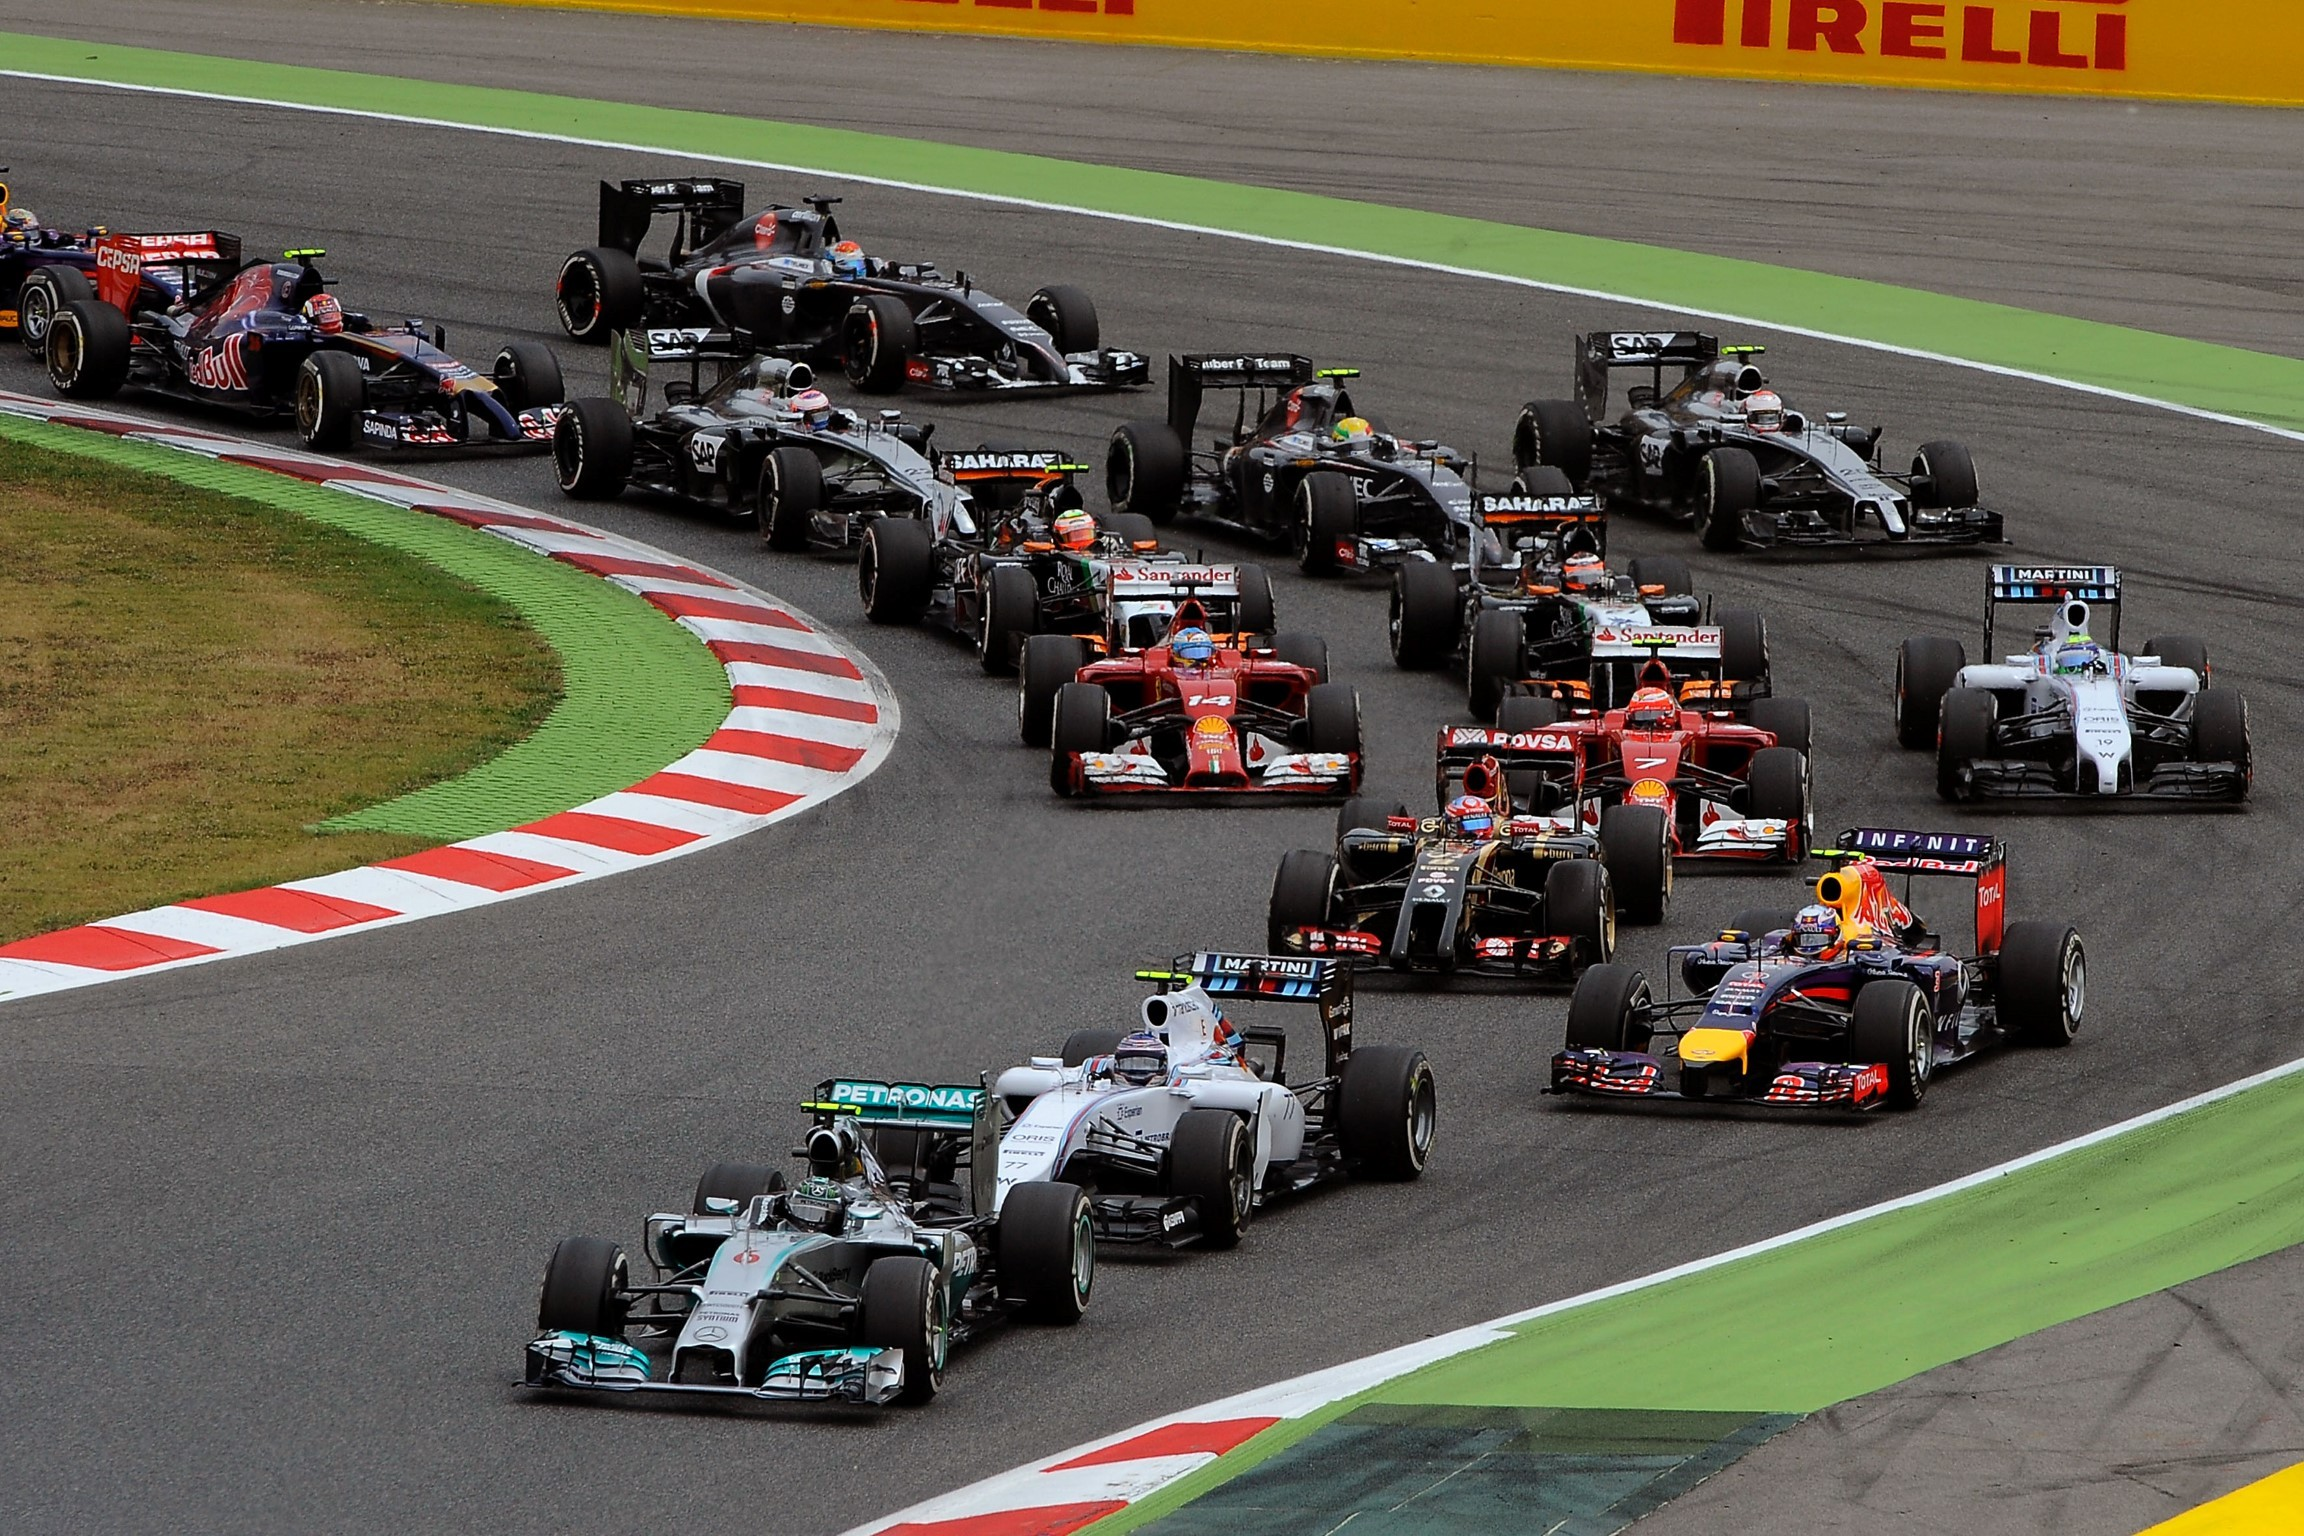
\includegraphics[width=\linewidth]{figs/parallelism.png}
\caption*{parallelism}
\end{figure}
\end{columns}
\end{frame}


%*******************************************************************************
%******************************* Frame *****************************************
%*******************************************************************************
\begin{frame}{Flynn's Classical Taxonomy}

\begin{figure}
\includegraphics[width=0.7\linewidth]{figs/flynn}
\caption*{Computer architecture}
\end{figure}
\end{frame}

%*******************************************************************************
%******************************* Frame *****************************************
%*******************************************************************************
\begin{frame}{Cost of parallelisation}
\begin{columns}

\column{0.49\linewidth}
$speedup = \frac{1}{1 - \mathrm{parallel part}}$
\begin{figure}
\includegraphics[width=\linewidth]{figs/amdahl1}
\caption*{Single processor}
\end{figure}
\column{0.49\linewidth}
$speedup = \frac{1}{\frac{\mathrm{parallel part}}{\mathrm{\# processors}} + 
\mathrm{serial part}}$
\begin{figure}
\includegraphics[width=\linewidth]{figs/amdahl2}
\caption*{Multiple processor}
\end{figure}
\end{columns}

Problems that increase the percentage of parallel time with their size are more 
\textbf{\textit{scalable}} than problems with a fixed percentage of parallel time

\end{frame}


%*******************************************************************************
%******************************* Frame *****************************************
%*******************************************************************************
\begin{frame}{Scalability}
\begin{itemize}
\item \textit{Strong scaling:} The total problem size stays fixed as more processors 
are added. 
\item \textit{Weak scaling:} The problem size per processor stays fixed as more 
processors are added. 

\item Simply adding more processors is rarely the answer to scalability.

\item The algorithm may have inherent limits to scalability. At some point, adding 
more resources causes performance to decrease. 

\item Hardware factors play a significant role in scalability. Examples:

\begin{itemize}
\item Memory-cpu bus bandwidth on Symmetric Multi-Processor (SMP) -
    where multiple processors share a single 
    address space and have equal access to all resources. 
\item Communications network bandwidth
\item Amount of memory available on any given machine or set of machines
\item Processor clock speed 

\end{itemize}

\item Parallel support libraries and subsystems software can limit scalability 
independent of your application. 
\end{itemize}

\end{frame}

\end{document}